\label{sec:Res}
\section*{Results}

\subsection*{Constant environment and density-dependence}

We used the previously developed model in \citetext{Sandell et al. 2014, master's thesis} and simulated (see~\autoref{fig:dd}) a tree population for 150 years in a constant environment, with and without density-dependence on $s_0$, assess the effects of a more realistic demography.

As expected, density-dependence allow regulating the population (\autoref{fig:dd} right panel), as the number of mature and immature individuals seem to converge respectively to $18000$ and $10000$ individuals, while without density-dependence the population is exponentially growing.

Looking at the phenotype, we started from exactly the same starting point $z=116$ for phenotypic and genotypic values. Without density-dependence, the population quickly converge to the equilibrium phenotype ($\overline{z_{weak}}$ given by the approximation in~\autoref{eq:zweak}), $\overline{z_{weak}} = 116$ in this case. With density-dependence the equilibrium is shifted towards the survival optimum $\theta_s$ ($\overline{z_{weak, dd}} = 121.8$, $\theta_s = 130$ while $\theta_f = 100$).

The lower seed survival $s_0$ decreases $\gamma_f$~\eqref{eq:gammaf} changing the weights in~\eqref{eq:zweak}, making it more interesting to favor the survival of already established immature trees than the production of many propagules with very little survival prospect.

Within the density-dependent model the mean immature phenotype $\overline{z_I}$ converge quicker than the mean mature phenotype $\overline{z_M}$ to the equilibrium. It is because of stage-structured nature of our model, the mature stage is a combination of individuals that lived for around 40 generations (given our life-cycle), it buffers adaptation. To make $\overline{z_M}$ closer to $\overline{z_{weak}}$, immature individuals with a phenotype closer to $\overline{z_{weak}}$ need to survive long enough to mature and outnumber initial mature individuals with phenotype further from $\overline{z_{weak}}$.

\subsection*{Fluctuating optima}

To mimic a changing environment we made the optima fluctuate (\autoref{fig:corr}, dashed lines) and compared this model to the one in constant environment (solid lines).

The mean phenotype of the population does not change very much with the fluctuations, indeed, $\overline{z_M}$ in constant and fluctuating environment are equal, and they are also equal to $\overline{z_{eq}}$, that is why they are indistinguishable on \autoref{fig:corr}.

Only $\overline{z_I}$ fluctuates under varying environment, but the fluctuations have a very small variance compared to the ones of the optima. We found a good correlation between fluctuating $\theta_s$ and $\overline{z_I}$ ($\rho_{\text{Pearson}} = 0.6997364$), no other correlation between $\theta_f$ or $\overline{z_M}$ are as high as this one. It shows how immature individuals track very smoothly the variations of the survival optimum and invest specifically more on this one.

Because of the variations, the mean of $s_I$ in fluctuating environment is lower than in constant environment, it explains why the number of immature individuals $N_I$ is lower under the fluctuating regime thus decreasing the number of mature individuals $N_M$, in the end it increases $s_0$ by density-dependence. The variation in $\theta_s$ causes $s_I$ to decrease, it underlines the cost of the fluctuations demographically: fluctuating regime causes variations in survival that may have dramatic effect on population.

However, those fluctuations do not seem to affect fecundities $f_1$ and $f_2$ in the same way (\autoref{fig:corr} bottom left panel). As the mean optima move they get closer to population phenotype increasing fecundity, but the next time step they move further away from this phenotype and they decrease fecundity.

The asymmetry of responses between, from the one hand, $s_I$, and from the other hand, $f_1$ and $f_2$, can be explained by the specific trade-off occurring in our population. The mean phenotype in our simulations is closer to $\theta_s$ than to $\theta_f$, there is a higher chance of $\theta_s$ to be lower or much higher than the mean population phenotype, then there is for $\theta_f$ to cross the mean population phenotype line.

As we had partially correlated noises in our population (see \autoref{tab:params} to have standard parameters set), we vary correlations for noises between 0 and 1. The results where consistent whatever the correlation coefficient. It seemed that the lower the correlation between noises, the higher were the demographic burden. Uncorrelated environments decrease more the life-history traits than correlated environments.

\subsection*{Trend in the environment}

We implemented a decreasing trend in $\theta_f$ with fluctuations (\autoref{fig:trend}) to mimic climate change.
We averaged values over 15 simulations for life-history traits while showed a single simulation for the phenotype (respectively bottom and top panels \autoref{fig:trend}).

$s_I$ has an interesting behavior, it first increases, reaches a maximum, then decreases. The decreasing trend in optima variation causes at first the mean population phenotype to move closer to $\theta_s$, thus maximizing $s_I$ values when it crosses $\theta_s$ line, as soon as it moves beyond $s_I$ starts to decrease again. The fluctuations seem to decrease $s_I$ (mean difference of 0.5), it may be a cost associated with the variance of optimum fluctuations, the optimum is often under the mean population value.

On the contrary $f_1$ and $f_2$ do not show a different pattern with or without fluctuations. They decrease because the mean population phenotype go further away from $\theta_f$.

Seed germination and survival $s_0$ is increased by fluctuations, via an indirect mechanism: fluctuations decrease immature survival $s_I$, thus decreasing the immature population $N_I$ and so the mature population $N_M$; this population decrease also decrease competition and density, increasing $s_0$ as it is density-dependent (see~\autoref{eq:ddfunc}).

As expected, the decreasing trend in $\theta_f$ creates a lag between the optima and the mean population values, because adaptation is slower than the rate of change. However, the population can still survive with such a rate if the difference between the optima and the means become constant. On a very long scale (2500 years) it is what happens in this case, the population maintain by changing its phenotype fast enough to track the optima variation (data not shown).

\subsection*{Estimation of the fluctuations}

In 6 localities (map \autoref{fig:thetaf} bottom left) using \textsc{PHENOFIT} output, we computed $\theta_f$ values at these locations (top 3 rows of \autoref{fig:thetaf}). For the 6 sites, predicted $\theta_f$ decrease with time, it is more precocious as time passes. This observation matches the advance of phenology observed in the literature because of climate change.

Over the general trend, we observe a small amplitude variation (with a standard deviation of \SI{9.6}{\day}), corresponding to year to year change in $\theta_f$ and some dramatic decreases in its values, sometimes reaching negative values (For example at BIC site in 1976). The frequency of these events increase with time as they become common after 2050 for all sites. Note that those events are biased towards the decrease of $\theta_f$, as there is no equivalent dramatic increases.

The negative values of $\theta_f$ computed in \autoref{fig:thetaf}, may seem striking as there is no such thing as a negative bud-burst date! It indicates strong directional selection to shorten bud-burst those years with very little sign of quadratic selection on that trait. As bottom right panel of \autoref{fig:thetaf} shows, we can have negative value of $\theta_f$ and still have achievable phenotypes. If $\theta_f$ is very negative for a given year (less than -100 in 2048 for LAB), it means there will be no reproduction this year (flat tail of blue curve, bottom right oanel \autoref{fig:thetaf}).

We excluded those extreme events, taking all sites together, to estimate the trend in the variation of $\theta_f$ (see~\nameref{sec:M&M}). Using linear regression on $\theta_f$ with time, we found a rate of \SI{-0.15}{\day\per\year}, with normal residuals having a variance of \SI{105}{\day\squared} (data not shown, $R^2=0.2341$, $p<2\text{\sc{e}-}16$, $F=186.7$ with $611$ d.f.).

We investigated whether there was a break between years modeled from real data by \textsc{PHENOFIT} (before 2001) and years modeled using climate models with climate change included (from 2001). We performed the same regression as above ($\theta_f$ with time), without taking apart the extreme values, for all sites, splitting the data before 2001 and from 2001 (data no shown). For each site, the slope estimates was higher with extreme events.

\begin{figure}[ht!]
	\centering
	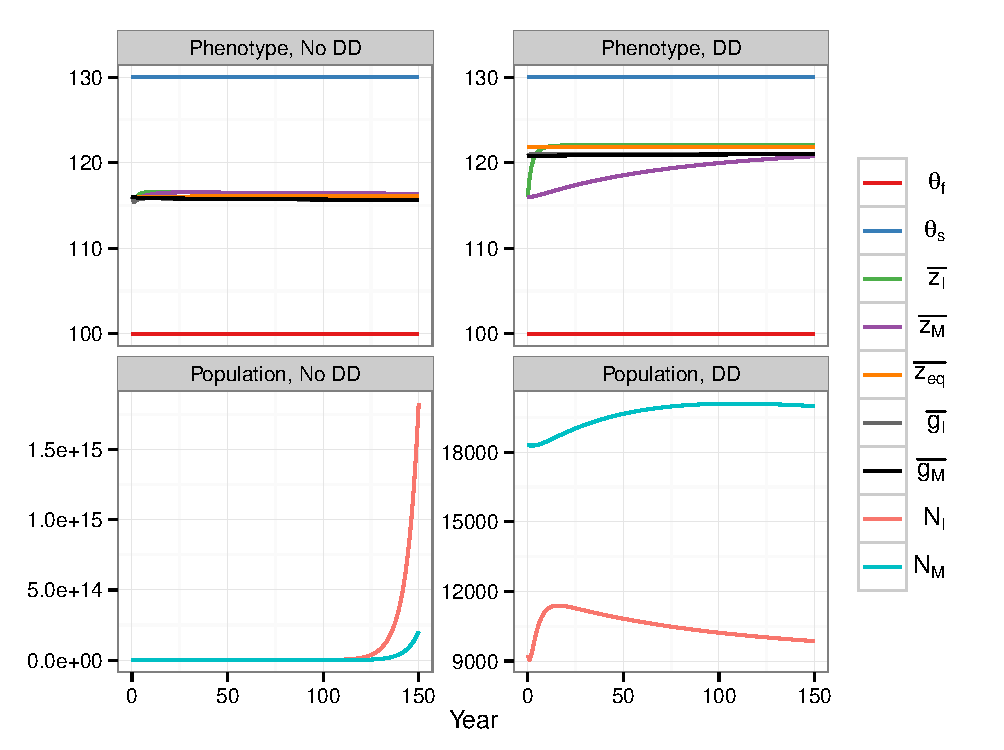
\includegraphics[scale=1]{Figures/DDphenopop.pdf}
	\caption{\textbf{Effect of density-dependence on phenotypes and populations}. \textbf{Top}: Phenotype variations in population ($\overline{z_I}, \overline{z_M}$, starting from $z = 116$) with their corresponding genotypic values ($\overline{g_I}, \overline{g_M}$), and the approximation given by \autoref{eq:zweak}; \textbf{Bottom}: Population, number of immature individuals ($N_I$, red), number of mature individuals ($N_M$, blue). Starting from Stable-Stage Distribution (SSD) in constant environment. \textbf{No DD} means we used the model without density-dependence, \textbf{DD} means we implemented density-dependence through $s_0$ (see \autoref{eq:ddfunc}).}
	\label{fig:dd}
\end{figure}

\begin{figure}[ht!]
	\centering
	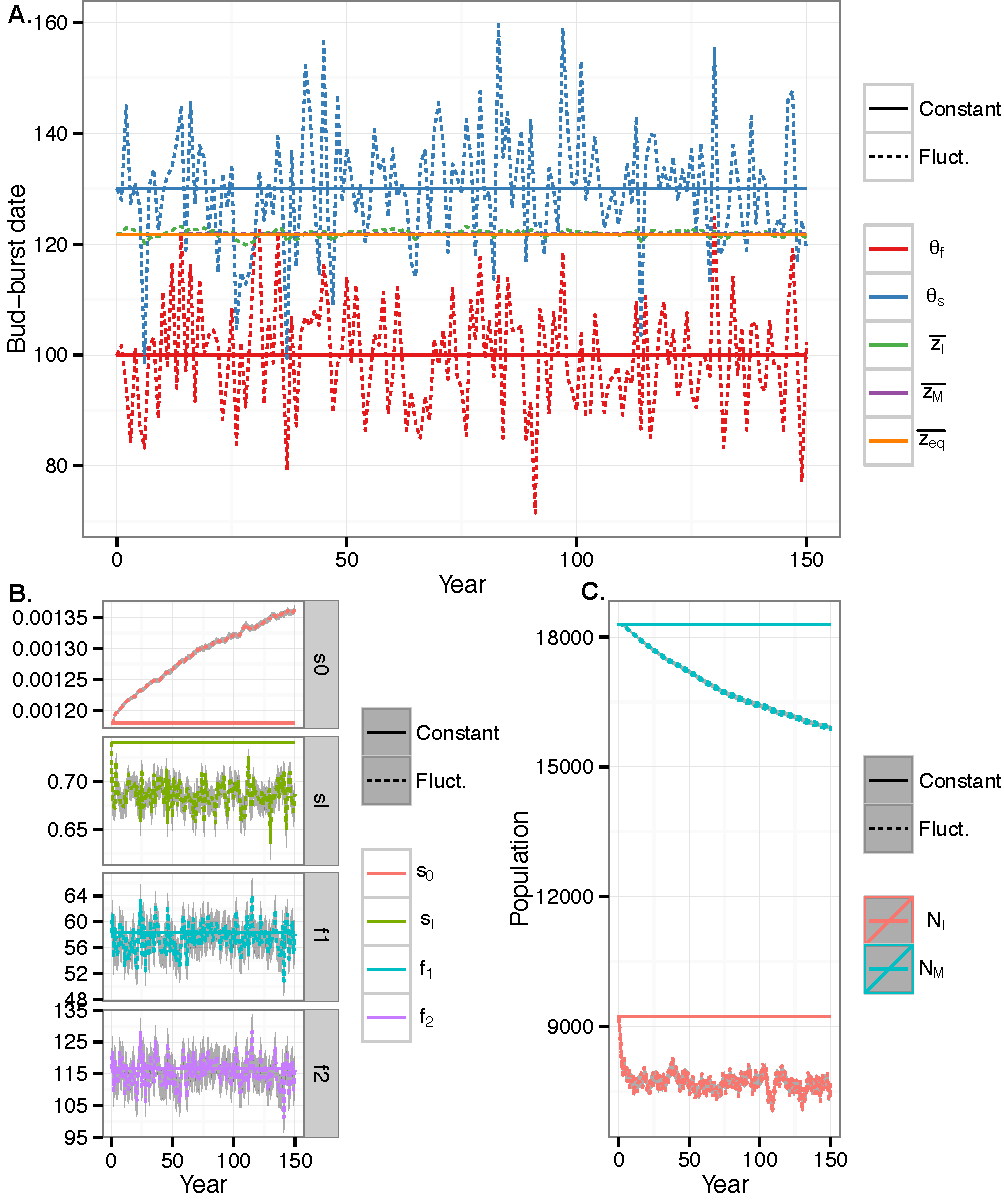
\includegraphics[scale=1]{Figures/PhenoLHTwithCorr.pdf}
	\caption{\textbf{Fluctuating optima against constant environment}. \textbf{Top:} comparison of phenotypes from simulations with constant or fluctuating optima, $\overline{z_{eq}}$ is the approximation shown in \autoref{eq:zweak}. \textbf{Bottom:} (\textbf{Left}) life-history traits in constant or fluctuating environment, (\textbf{Right}) population in constant or fluctuating environment, $N_I$ is the number of immature individuals and $N_M$ the number of mature individuals, population started from the stable stage distribution. \textbf{Solid lines:} values in constant environment, \textbf{Dashed lines:} in fluctuating environment.}
	\label{fig:corr}
\end{figure}

\begin{figure}[ht!]
	\centering
	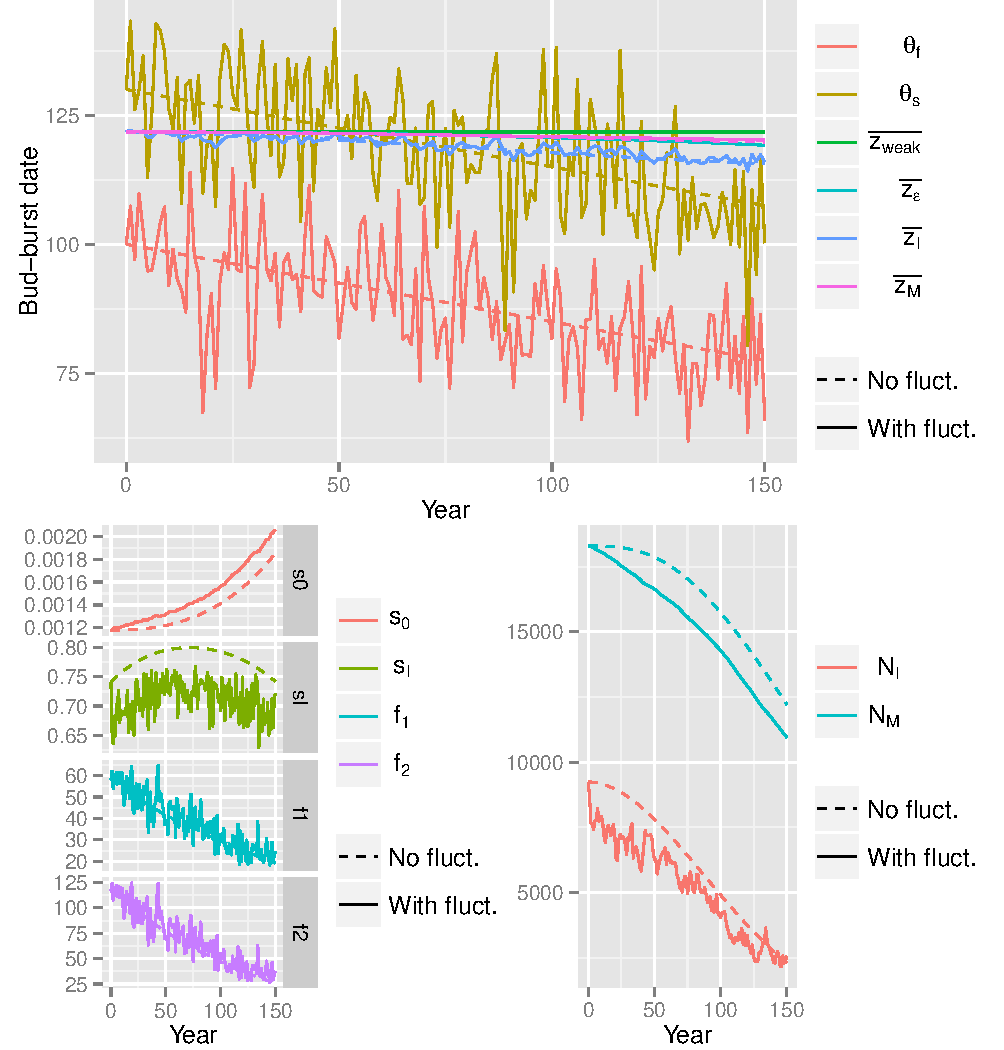
\includegraphics[scale=1]{Figures/Trend.pdf}
	\caption{\textbf{Mixed influences of trend and fluctuations on the population}. \textbf{Top:} Phenotype evolution with and without fluctuations, results from a \textbf{single} simulation; \textbf{Bottom:} (\textbf{Left}) life-history traits evolution; (\textbf{Right}) demography. \textbf{Solid lines:} (\textbf{No fluct.}) linearly decreasing optima with time; \textbf{Dashed lines:} \textbf{With fluct.} fluctuating decreasing optima. Life-history traits and population were averaged over 15 independent population to buffer the stochasticity of simulations.}
	\label{fig:trend}
\end{figure}

\begin{figure}[ht!]
	\centering
	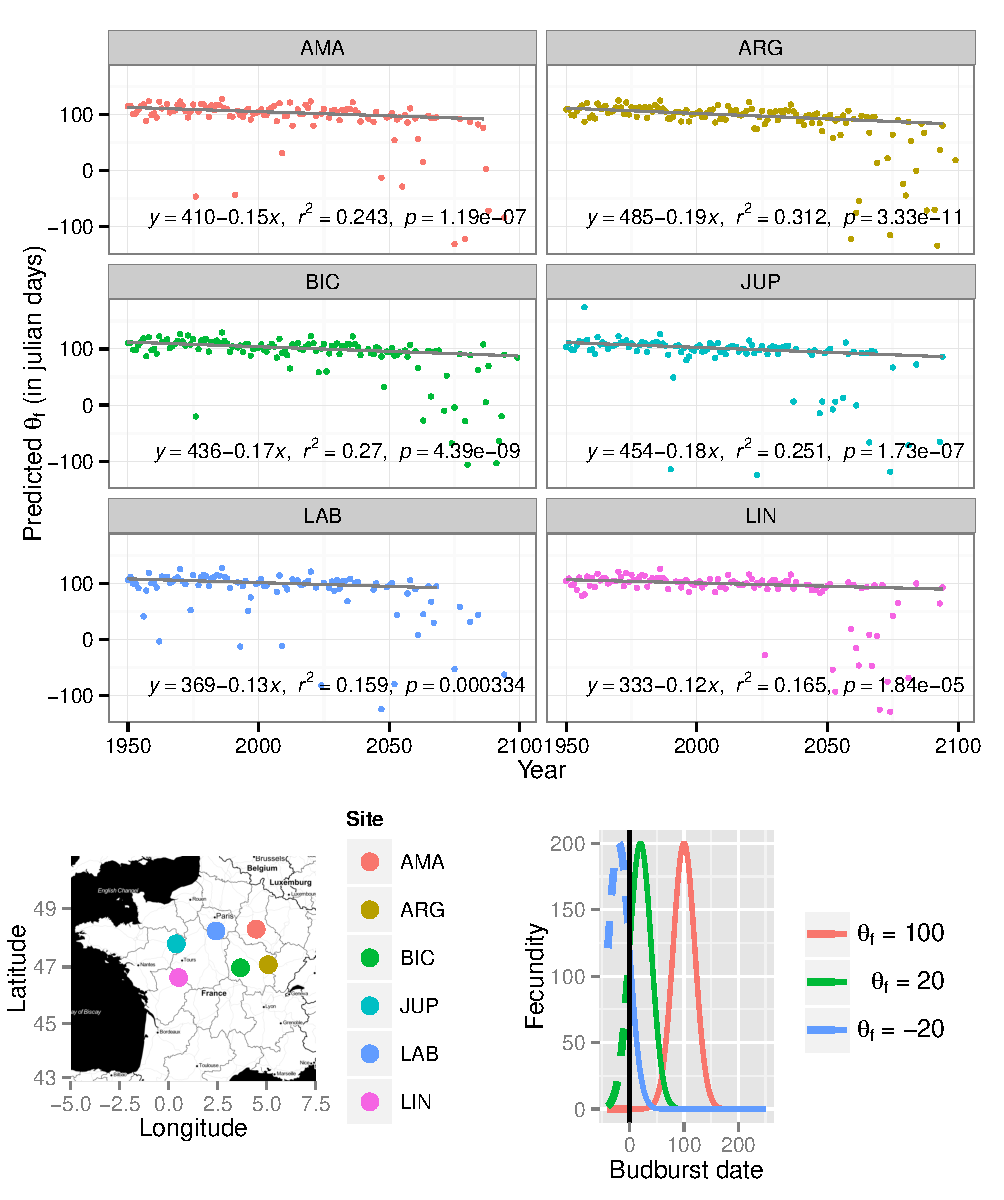
\includegraphics[scale=1]{Figures/optsmaps.pdf}
	\caption{\textbf{$\theta_{f}$ estimations from PHENOFIT data}. \textbf{Top:} estimations of $\theta_f$ for each study site (see \nameref{sec:M&M} for details). \textbf{Bottom:} (\textbf{Left}) map of the study sites; (\textbf{Right}) Theoretical fecundity functions with parameters from~\autoref{tab:params} with values of $\theta_f$ equals to $100$, $20$ and $-20$, solid lines indicate achievable phenotype, dashed lines show theoretical curves but unreachable phenotypes.}
	\label{fig:thetaf}
\end{figure}